\documentclass[final,3p,authoryear]{elsarticle}

\usepackage{lipsum}
 \usepackage{graphics}
\usepackage[]{algorithm2e}
 \usepackage{setspace}
%% or use the graphicx package for more complicated commands
 \usepackage{graphicx}
%% or use the epsfig package if you prefer to use the old commands
 \usepackage{epsfig}
 \usepackage{subfigure}

%% The amssymb package provides various useful mathematical symbols
\usepackage{amssymb}
%% The amsthm package provides extended theorem environments
 \usepackage{amsthm,amsmath}
 \usepackage{multirow}
 \usepackage{setspace}
 \usepackage{CJK}
 \usepackage{float}
 \usepackage{pdfpages}
 \usepackage{mathtools}
% \usepackage{natbib}
 \restylefloat{table}
 \onehalfspacing



\makeatletter
\def\ps@pprintTitle{%
	\let\@oddhead\@empty
	\let\@evenhead\@empty
	\def\@oddfoot{}%
	\let\@evenfoot\@oddfoot}
\makeatother

\usepackage{etoolbox}
\patchcmd{\abstract}{Abstract}{}{}{}

\begin{document}

\begin{frontmatter}

\title{MATH 6740: Financial Mathematics and Simulation\\
	Homework 4 solutions/presentation}

\author[rvt]{Jubiao ``Jack'' Yang}

\address[rvt]{Rensselaer Polytechnic Institute, Troy, NY 12180}

\begin{abstract}
	Solve Exercise Problems 2.5 and 2.10 in \cite[Chapter 2]{shreve2004stochastic}, and Problems 3.1, 3.2, and 3.4 in \cite[Chapter 3]{shreve2004stochastic}.
\end{abstract}


\end{frontmatter}

\section{Exercise 2.5}
	The p.d.f. for random variable $X$ is:
	\begin{eqnarray}
		f_X(x) &=& \int_{-\infty}^{+\infty} f_{X,Y}(x,y) dy \nonumber\\
		&=& \int_{-\left|x\right|}^{+\infty} \frac{2\left|x\right|+y}{\sqrt{2\pi}} \exp\left\{-\frac{\left(2\left|x\right|+y\right)^2}{2}\right\} dy \nonumber\\
		&=& \frac{1}{\sqrt{2\pi}} \int_{-\left|x\right|}^{+\infty} \left(2\left|x\right|+y\right) \exp\left\{-\frac{\left(2\left|x\right|+y\right)^2}{2}\right\} d\left(2\left|x\right|+y\right) \nonumber\\
		&=& \frac{1}{\sqrt{2\pi}} \int_{-\left|x\right|}^{+\infty} \exp\left\{-\frac{\left(2\left|x\right|+y\right)^2}{2}\right\} d\frac{\left(2\left|x\right|+y\right)^2}{2} \nonumber\\
		&=& \frac{1}{\sqrt{2\pi}} \left( \exp\left\{-\frac{\left|x\right|^2}{2}\right\} - \exp\left\{ -\infty \right\} \right)
		= \frac{1}{\sqrt{2\pi}} \exp\left\{-\frac{x^2}{2}\right\}
		,
	\end{eqnarray}
	and the p.d.f. for random variable $Y$ is:
	\begin{eqnarray}
		f_Y(y) &=& \int_{-\infty}^{+\infty} f_{X,Y}(x,y) dx \nonumber\\
		&=& 2 \int_{0}^{+\infty} \frac{2\left|x\right|+y}{\sqrt{2\pi}} \exp\left\{-\frac{\left(2\left|x\right|+y\right)^2}{2}\right\} dx \nonumber\\
		&=& \frac{2}{\sqrt{2\pi}} \int_{\max\{0,-y\}}^{+\infty} \left(2x+y\right) \exp\left\{-\frac{\left(2x+y\right)^2}{2}\right\} dx \nonumber\\
		&=& \frac{1}{\sqrt{2\pi}} \int_{\max\{0,-y\}}^{+\infty} \exp\left\{-\frac{\left(2x+y\right)^2}{2}\right\} d\frac{\left(2x+y\right)^2}{2} \nonumber\\
		&=& \frac{1}{\sqrt{2\pi}} \left( \exp\left\{-\frac{\left(2\max\{0,-y\}+y\right)^2}{2}\right\} -0 \right) \nonumber\\
		&=& \frac{1}{\sqrt{2\pi}} \exp\left\{-\frac{\left|y\right|^2}{2}\right\}
		= \frac{1}{\sqrt{2\pi}} \exp\left\{-\frac{y^2}{2}\right\}
		.
	\end{eqnarray}
	Therefore both $X$ and $Y$ are standard normal random variables. The covariance of them is:
	\begin{eqnarray}
		cov(X,Y) &=& E[\left(X-E[X]\right)\left(Y-E[Y]\right)] = E[XY] \nonumber\\
		&=& \int_{-\infty}^{+\infty} \int_{-\infty}^{+\infty} xy f_{X,Y}(x,y) dx dy \nonumber\\
		&=& \int_{-\infty}^{+\infty} y \left( \int_{-\infty}^{+\infty} x \frac{2\left|x\right|+y}{\sqrt{2\pi}} \exp\left\{-\frac{\left(2\left|x\right|+y\right)^2}{2}\right\} dx \right) dy \nonumber\\
		&=& \int_{-\infty}^{+\infty} y \cdot 0 dy =0
		,
	\end{eqnarray}
	therefore $X$ and $Y$ are uncorrelated. However, since $f_{X,Y}(x,y) \neq f_X(x) f_Y(y)$, $X$ and $Y$ are not independent.
	
\section{Exercise 2.10}
	\begin{eqnarray}
		\int_{A} g(X) dP(X) &=& \int_{-\infty}^{+\infty} g(x) 1_{\omega \in A} f_X(x) dx \nonumber\\
		&=& \int_{-\infty}^{+\infty} \left( \int_{-\infty}^{+\infty} \frac{y f_{X,Y}(x,y)}{f_{X}(x)} dy \right) 1_{\omega \in A} f_X(x) dx \nonumber\\
		&=& \int_{-\infty}^{+\infty} \left( \int_{-\infty}^{+\infty} y f_{X,Y}(x,y) dy \right) 1_{\omega \in A} dx \nonumber\\
		&=& \int_{-\infty}^{+\infty} y \left( \int_{-\infty}^{+\infty} f_{X,Y}(x,y) dx \right) 1_{\omega \in A} dy \nonumber\\
		&=& \int_{-\infty}^{+\infty} y 1_{\omega \in A} f_Y(y) dy = \int_{A} Y dP(Y)
		.
	\end{eqnarray}

\section{Exercise 3.1}
	According to Definition 3.3.3(iii) in \citet{shreve2004stochastic}, $W(u_2)-W(u_1)$ is independent of $\mathbb{F}(u_1)$; while according to Definition 3.3.3(i) in \citet{shreve2004stochastic}, $\mathbb{F}(t) \subset \mathbb{F}(u_1)$. Therefore $W(u_2)-W(u_1)$ is independent of $\mathbb{F}(t)$.
	
\section{Exercise 3.2}
	For $0\leq s \leq t$:
	\begin{eqnarray}
		E[W^2(t)-t | \mathbb{F}_s] &=& E[\left( W(t)-W(s) \right)^2 + 2W(t)W(s) - W^2(s) -t | \mathbb{F}(s)] \nonumber\\
		&=& E[\left( W(t)-W(s) \right)^2] + 2W(s) E[W(t)-W(s)+W(s) | \mathbb{F}(s)] - W^2(s) - t \nonumber\\
		&=& var(W(t)-W(s)) + 2W(s) \left( W(s) + E[W(t)-W(s) | \mathbb{F}(s)] \right) - W^2(s) - t \nonumber\\
		&=& t-s + 2W^2(s) - W^2(s) - t \nonumber\\
		&=& W^2(s) - s
		,
	\end{eqnarray}
	therefore $\{ W^2(t)-t \}$ is a martingale.
	
\section{Exercise 3.4}
	\subsection{(i)}
		\begin{eqnarray}
			\sum\limits_{j=0}^{n-1} \left| W(t_{j+1}) - W(t_j) \right| \cdot \max\limits_{0 \leq k \leq n-1} \left| W(t_{j+1}) - W(t_j) \right|
			\geq 
			\sum\limits_{j=0}^{n-1} \left( W(t_{j+1}) - W(t_j) \right)^2
			,
		\end{eqnarray}
		therefore the first variation of Brownian motion is:
		\begin{eqnarray}
			\lim\limits_{|| \Pi || \to 0} \sum\limits_{j=0}^{n-1} \left| W(t_{j+1}) - W(t_j) \right|
			\geq
			\lim\limits_{|| \Pi || \to 0} \frac{\sum\limits_{j=0}^{n-1} \left( W(t_{j+1}) - W(t_j) \right)^2}{\max\limits_{0 \leq k \leq n-1} \left| W(t_{j+1}) - W(t_j) \right|}
			= \frac{T}{0} = \infty
			.
		\end{eqnarray}
	
	\subsection{(ii)}
		\begin{eqnarray}
			\sum\limits_{j=0}^{n-1} \left| W(t_{j+1}) - W(t_j) \right|^3
			\leq
			\max\limits_{0 \leq k \leq n-1} \left| W(t_{j+1}) - W(t_j) \right| \cdot \sum\limits_{j=0}^{n-1} \left| W(t_{j+1}) - W(t_j) \right|^2
			,
		\end{eqnarray}
		therefore the cubic variation of Brownian motion is:
		\begin{eqnarray}
			\lim\limits_{|| \Pi || \to 0} \sum\limits_{j=0}^{n-1} \left| W(t_{j+1}) - W(t_j) \right|^3
			\leq
			\lim\limits_{|| \Pi || \to 0} \max\limits_{0 \leq k \leq n-1} \left| W(t_{j+1}) - W(t_j) \right| \cdot \lim\limits_{|| \Pi || \to 0} \sum\limits_{j=0}^{n-1} \left| W(t_{j+1}) - W(t_j) \right|^2 \nonumber\\
			= 0 \cdot T =0
		\end{eqnarray}
	

	
\appendix

\section{Original Homework Questions (attached)}
%	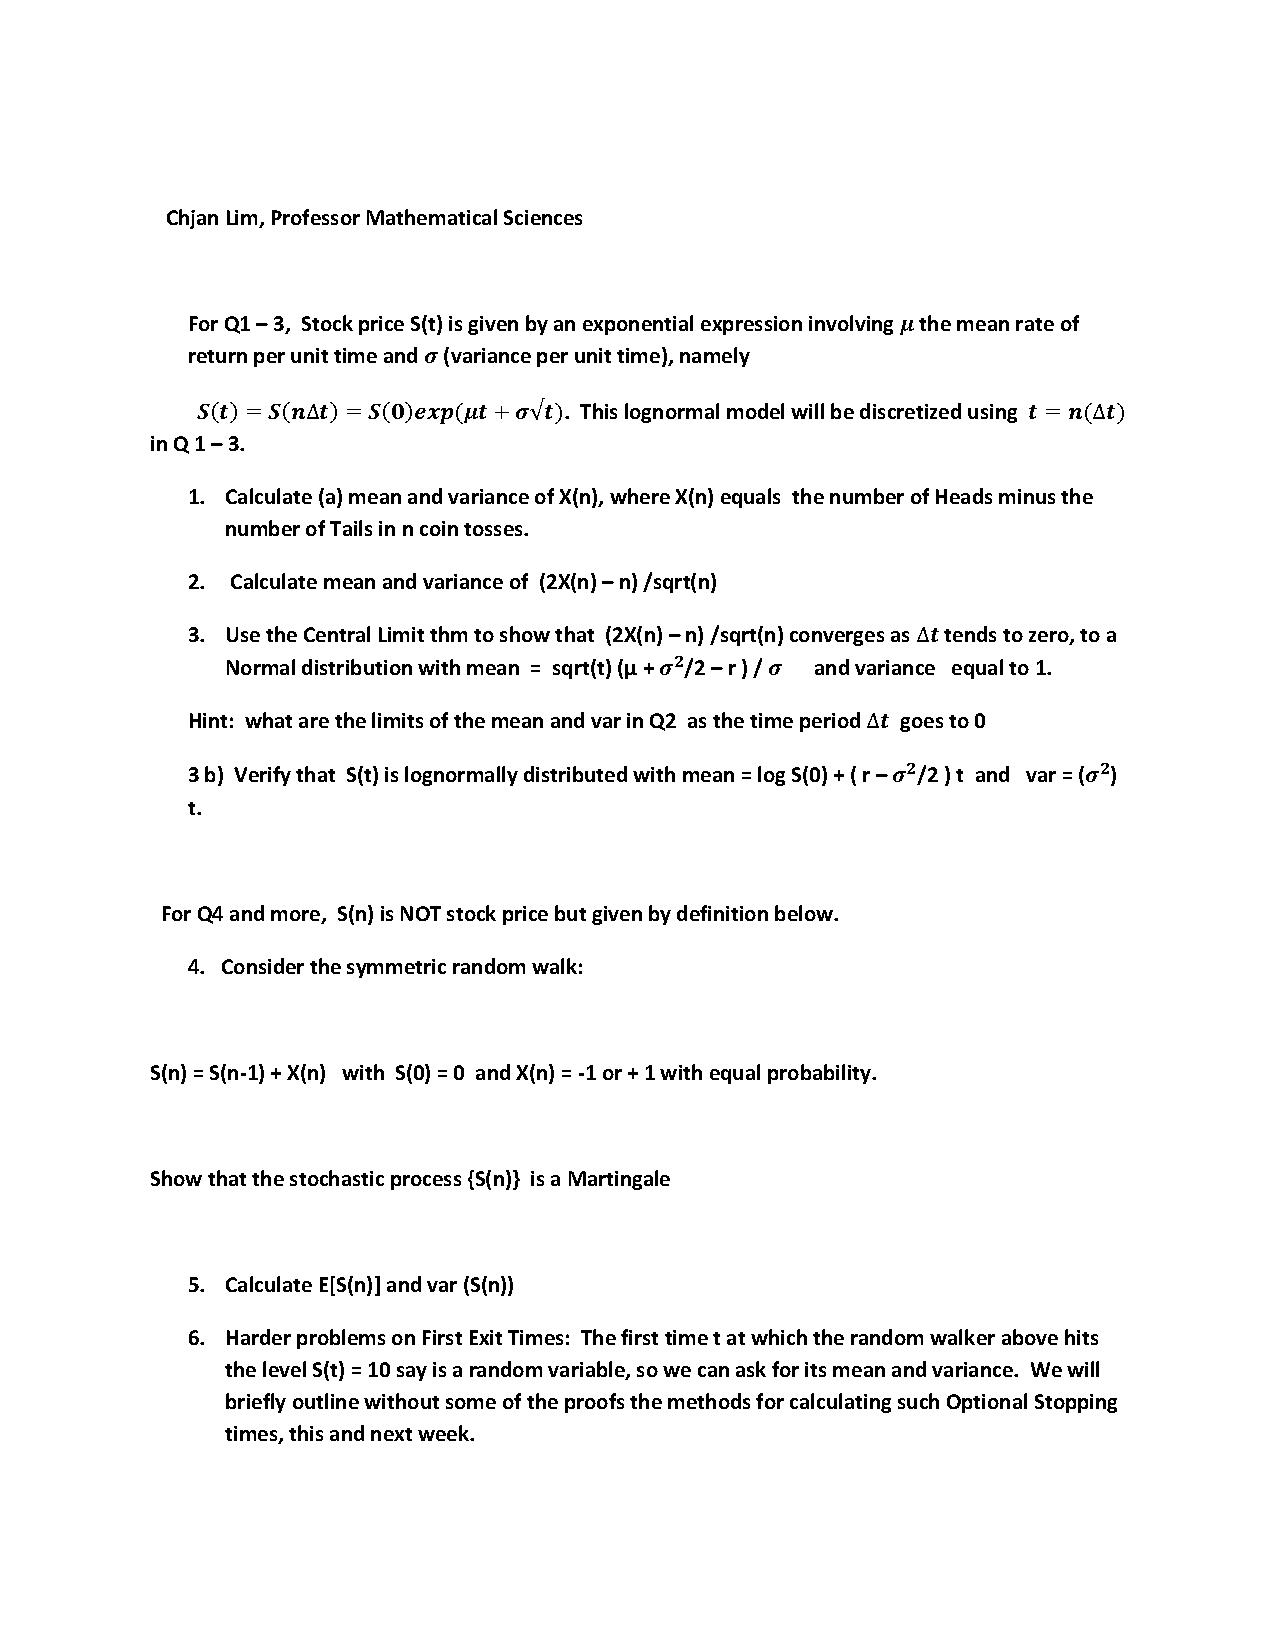
\includepdf[pages={1}]{worksheet216.pdf}
	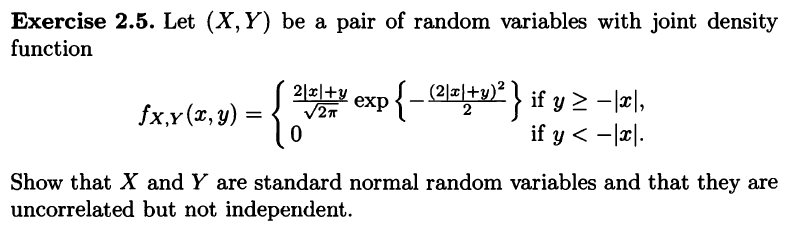
\includegraphics[width=14cm]{Ex2p5.png}\\
	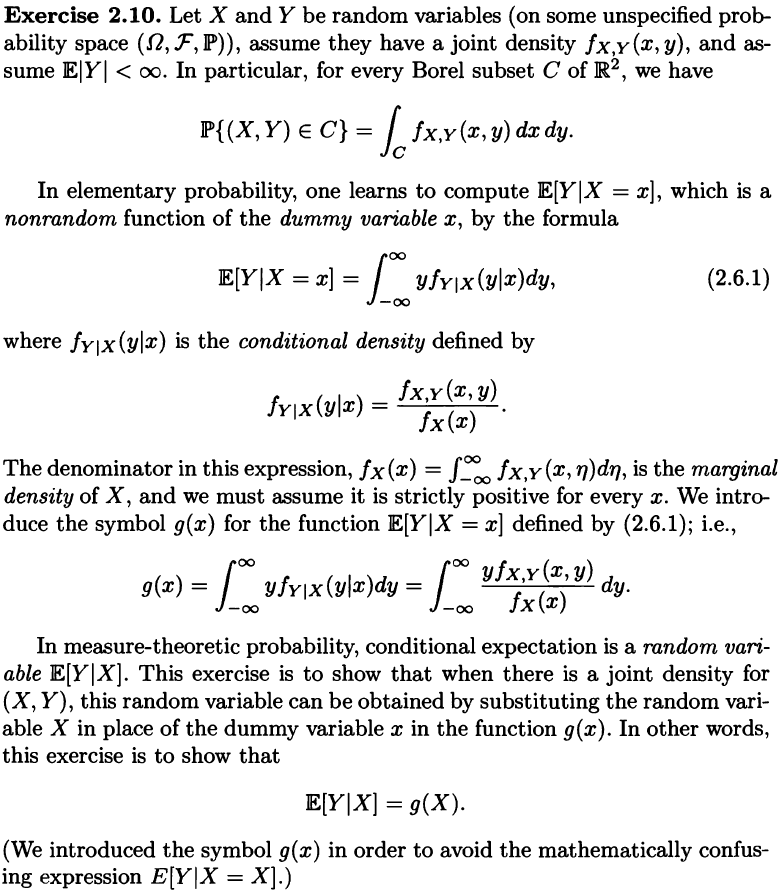
\includegraphics[width=14cm]{Ex2p10s1.png}\\
	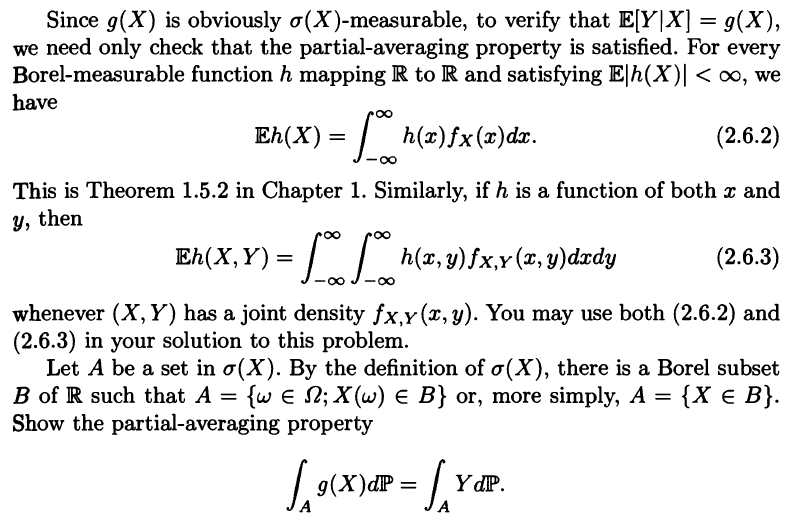
\includegraphics[width=14cm]{Ex2p10s2.png}\\
	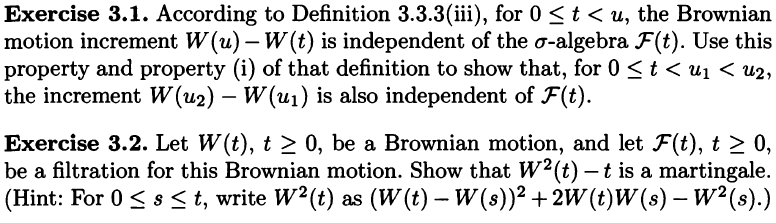
\includegraphics[width=14cm]{Ex3p1a3p2.png}\\
	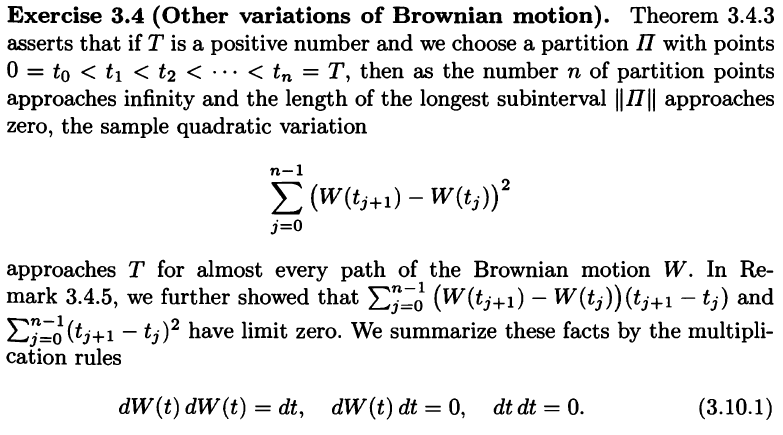
\includegraphics[width=14cm]{Ex3p4s1.png}\\
	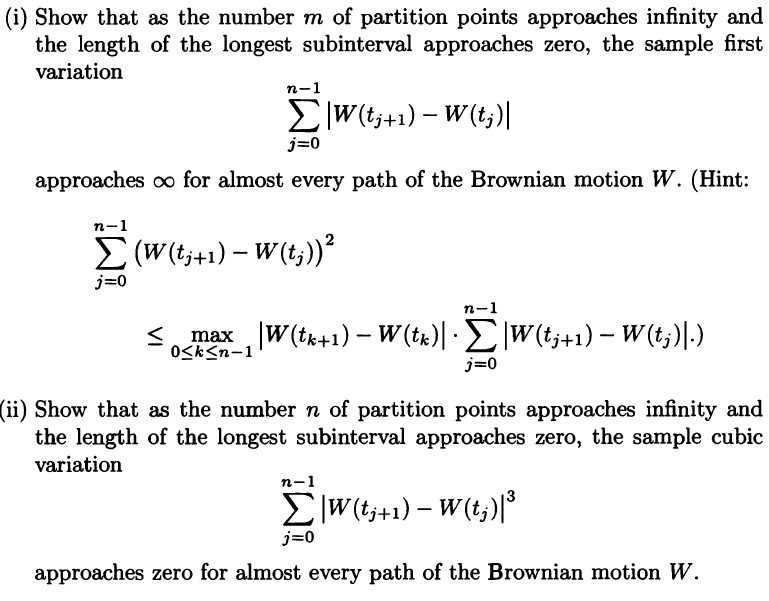
\includegraphics[width=14cm]{Ex3p4s2.png}


%	\appendix
%%% \section{}
%%% \label{}
%
%%% References
%%%
%%% Following citation commands can be used in the body text:
%%% Usage of \cite is as follows:
%%%   \cite{key}         ==>>  [#]
%%%   \cite[chap. 2]{key} ==>> [#, chap. 2]
%%%
%
%%% References with bibTeX database:
%
%	\section{Reference}
	\bibliographystyle{elsarticle-harv}
	\bibliography{../MATH6740cit}
%
%%% Authors are advised to submit their bibtex database files. They are
%%% requested to list a bibtex style file in the manuscript if they do
%%% not want to use elsarticle-num.bst.
%
%%% References without bibTeX database:
%
%% \begin{thebibliography}{00}
%
%%% \bibitem must have the following form:
%%%   \bibitem{key}...
%%%
%
%% \bibitem{}
%
%% \end{thebibliography}

\end{document}



